\documentclass[12pt, a4paper]{article}
\usepackage{../../../myconfig} % Gọi file cấu hình từ ngoài gốc vào
% ==========================================
% BẮT ĐẦU NỘI DUNG TÀI LIỆU
% ==========================================
\begin{document}

% Truyền 3 tham số: {Nhãn cam} {Chữ to chính giữa} {Chữ ở góc phải Header}
\titlebox{Chủ đề: Tích phân}{Ứng dụng tích phân trong bài toán chuyển động}{Bài toán chuyển động}

% --- CÂU 1 ---
\questionTrueFalse{0}{1}{Một xe ô tô đang chạy với vận tốc 72 km/h thì người lái xe bất ngờ phát hiện chướng ngại vật trên đường cách đó 100 m. Người lái xe phản ứng mất 2 giây, sau đó đạp phanh khẩn cấp. Kể từ thời điểm này, ô tô chuyển động chậm dần đều với vận tốc \(v(t) = -4t + 20\) (m/s), trong đó \(t\) là thời gian tính bằng giây kể từ lúc đạp phanh. Gọi \(s(t)\) là quãng đường xe ô tô đi được trong \(t\) giây kể từ lúc đạp phanh.}{
    \textbf{a)} & Quãng đường \(s(t)\) mà xe ô tô đi được trong thời gian \(t\) giây là một nguyên hàm của hàm số \(v(t)\).
    & \textcolor{amberorange}{$\bigcirc$} & \textcolor{amberorange}{$\bigcirc$} \\ \hline
    
    \textbf{b)} & \(s(t) = -4t^2 + 16t\).
    & \textcolor{amberorange}{$\bigcirc$} & \textcolor{amberorange}{$\bigcirc$} \\ \hline
    
    \textbf{c)} & Thời gian kể từ lúc đạp phanh đến khi xe ô tô dừng hẳn là 3 giây.
    & \textcolor{amberorange}{$\bigcirc$} & \textcolor{amberorange}{$\bigcirc$} \\ \hline
    
    \textbf{d)} & Kể từ lúc đạp phanh đến khi xe ô tô dừng hẳn thì xe ô tô đó không va vào chướng ngại vật ở trên đường.
    & \textcolor{amberorange}{$\bigcirc$} & \textcolor{amberorange}{$\bigcirc$} \\
}

% --- CÂU 2 ---
\questionTrueFalse{0}{2}{Chất điểm chuyển động theo quy luật vận tốc \(v(t)\) (m/s) có dạng đường Parabol \(v(t) = t^2 + bt + c\) khi \(0 \leq t \leq 4\) và \(v(t)\) có dạng đường thẳng khi \(4 \leq t \leq 8\). Đồ thị \(v(t)\) được cho như hình bên.
\begin{center}
    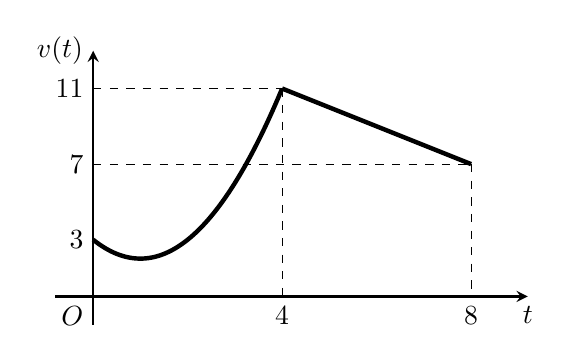
\begin{tikzpicture}[scale=0.6, >=stealth]
    % Tỷ lệ tọa độ: x = t, y = v / 2.5
    % t=0 (0, 1.2)      [v=3]
    % t=4 (4, 4.4)      [v=11]
    % t=8 (8, 2.8)      [v=7]

    % Trục tọa độ
    \draw[->, thick] (-0.8, 0) -- (9.2, 0) node[below] {$t$};
    \draw[->, thick] (0, -0.6) -- (0, 5.2) node[left] {$v(t)$};

    % Gốc tọa độ O
    \node[below left] at (0,0) {$O$};

    % Đường đứt nét (Dashed lines)
    \draw[dashed] (0, 4.4) node[left] {$11$} -- (4, 4.4);
    \draw[dashed] (0, 2.8) node[left] {$7$} -- (8, 2.8);
    
    \draw[dashed] (4, 4.4) -- (4, 0) node[below] {$4$};
    \draw[dashed] (8, 2.8) -- (8, 0) node[below] {$8$};

    % Giá trị v = 3
    \node[left] at (0, 1.2) {$3$};

    % Đồ thị
    % Đoạn 1: Parabol v(t) = t^2 - 2t + 3 trên [0, 4] -> y = (x^2 - 2x + 3)/2.5
    \draw[ultra thick, domain=0:4, samples=100] 
        plot (\x, {(\x*\x - 2*\x + 3)/2.5});

    % Đoạn 2: Đoạn thẳng nối từ (4, 11) đến (8, 7)
    \draw[ultra thick] (4, 4.4) -- (8, 2.8);

\end{tikzpicture}
\end{center}

}{
    \textbf{a)} & Giá trị của \(b = -2\).
    & \textcolor{amberorange}{$\bigcirc$} & \textcolor{amberorange}{$\bigcirc$} \\ \hline
    
    \textbf{b)} & Giá trị nhỏ nhất của \(v(t)\) trong 8 giây đầu tiên bằng 1 m/s.
    & \textcolor{amberorange}{$\bigcirc$} & \textcolor{amberorange}{$\bigcirc$} \\ \hline
    
    \textbf{c)} & Quãng đường vật đi được trong thời gian từ giây thứ 4 đến giây thứ 8 là 36 m.
    & \textcolor{amberorange}{$\bigcirc$} & \textcolor{amberorange}{$\bigcirc$} \\ \hline
    
    \textbf{d)} & Trong 8 giây đầu tiên, vật đi được quãng đường 53 m (kết quả làm tròn đến hàng đơn vị).
    & \textcolor{amberorange}{$\bigcirc$} & \textcolor{amberorange}{$\bigcirc$} \\
}

% --- CÂU 3 ---
\questionTrueFalse{0}{3}{Một chất điểm \(A\) chuyển động trên trục số \(Ox\), với vận tốc \(v(t) = 3t^2 - 24t + 46\) (m/s) trong đó thời điểm \(t = 0\) tính từ lúc chất điểm bắt đầu chuyển động và khi đó chất điểm ở tại gốc tọa độ.
\begin{center}
    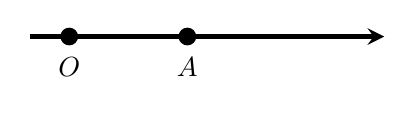
\begin{tikzpicture}[>=stealth]
    % Trục tọa độ Ox
    \draw[->,ultra thick] (0, 0) -- (4.5, 0);

    % Điểm O
    \filldraw (0.5, 0) circle (3pt) node[below=4pt] {$O$};

    % Điểm A
    \filldraw (2.0, 0) circle (3pt) node[below=4pt] {$A$};
\end{tikzpicture}
\end{center}
}{
    \textbf{a)} & Quãng đường chất điểm đi được trong 2 giây đầu tiên là 52 m.
    & \textcolor{amberorange}{$\bigcirc$} & \textcolor{amberorange}{$\bigcirc$} \\ \hline
    
    \textbf{b)} & Khoảng cách giữa vị trí của chất điểm tại thời điểm 5 giây và vị trí của chất điểm tại thời điểm ban đầu là 55 m.
    & \textcolor{amberorange}{$\bigcirc$} & \textcolor{amberorange}{$\bigcirc$} \\ \hline
    
    \textbf{c)} & Trong khoảng thời gian từ 3 giây tới 6 giây, tốc độ chất điểm lớn nhất là 8 m/s.
    & \textcolor{amberorange}{$\bigcirc$} & \textcolor{amberorange}{$\bigcirc$} \\ \hline
    
    \textbf{d)} & Tại thời điểm \(t = 0\), tại gốc tọa độ một chất điểm \(B\) khác chuyển động trên trục \(Ox\) với vận tốc \(v_B(t) = 14\) (m/s). Hai chất điểm \(A\) và \(B\) gặp nhau lần thứ hai cách thời điểm ban đầu là 8 giây (thời điểm \(t = 0\) được xem là thời điểm hai chất điểm gặp nhau lần thứ nhất).
    & \textcolor{amberorange}{$\bigcirc$} & \textcolor{amberorange}{$\bigcirc$} \\
}

% --- CÂU 4 ---
\questionTrueFalse{0}{4}{Một chất điểm \(A\) xuất phát từ \(O\), chuyển động thẳng với vận tốc biến thiên theo thời gian bởi quy luật \(v(t) = \dfrac{1}{150}t^2 + \dfrac{59}{75}t\) (m/s), trong đó \(t\) (giây) là khoảng thời gian tính từ lúc bắt đầu chuyển động. Từ trạng thái nghỉ, một chất điểm \(B\) cũng xuất phát từ \(O\), chuyển động thẳng cùng hướng với \(A\) nhưng chậm hơn 3 giây so với \(A\) và có gia tốc bằng \(a\) (m/s\(^2\)) (\(a\) là hằng số). Sau khi \(B\) xuất phát được 12 giây thì đuổi kịp \(A\).}{
    \textbf{a)} & Vận tốc của \(A\) tại thời điểm \(B\) đuổi kịp \(A\) là \(13,3\) m/s.
    & \textcolor{amberorange}{$\bigcirc$} & \textcolor{amberorange}{$\bigcirc$} \\ \hline
    
    \textbf{b)} & Khi \(B\) đuổi kịp \(A\) thì \(A\) đi được quãng đường 96 m.
    & \textcolor{amberorange}{$\bigcirc$} & \textcolor{amberorange}{$\bigcirc$} \\ \hline
    
    \textbf{c)} & Giá trị của \(a\) là \(\dfrac{4}{3}\).
    & \textcolor{amberorange}{$\bigcirc$} & \textcolor{amberorange}{$\bigcirc$} \\ \hline
    
    \textbf{d)} & Vận tốc của \(B\) tại thời điểm \(B\) đuổi kịp \(A\) là 16 m/s.
    & \textcolor{amberorange}{$\bigcirc$} & \textcolor{amberorange}{$\bigcirc$} \\
}

% --- CÂU 5 ---
\questionShortAnswer{0}{5}{Hai ô tô xuất phát tại cùng một thời điểm đi trên cùng đoạn thẳng \(AB\), ô tô thứ nhất bắt đầu xuất phát từ \(A\) và đi theo hướng từ \(A\) đến \(B\) với vận tốc \(v_1(t) = 4t + 2\) (km/h). Ô tô thứ hai xuất phát từ \(O\) cách \(A\) một khoảng 10 km và đi theo hướng từ \(A\) đến \(B\) với vận tốc 14 km/h, sau một khoảng thời gian người lái đạp phanh; từ thời điểm đó, ô tô thứ hai chuyển động chậm dần đều với vận tốc \(v_2(t) = -4t + 22\) (km/h). Hỏi sau khoảng thời gian bao nhiêu giờ kể từ khi xuất phát hai ô tô đó gặp nhau (làm tròn kết quả đến hàng phần trăm)?
}

% --- CÂU 6 ---
\questionShortAnswer{0}{6}{Một vật bắt đầu chuyển động thẳng đều với vận tốc \(v_0 = a\) (m/s) với \(a > 0\). Sau 6 giây chuyển động thì gặp chướng ngại vật nên bắt đầu giảm tốc độ với vận tốc \(v(t) = -\dfrac{5}{2}t + b\) (m/s), (\(t \geq 6\)) cho đến khi dừng hẳn. Biết rằng, kể từ lúc chuyển động đến lúc dừng thì vật đi được quãng đường là 80 (m). Giá trị của \(a^2 - b^2\) bằng bao nhiêu?
}

% --- CÂU 7 ---
\questionShortAnswer{0}{7}{Một vật đang chuyển động đều với vận tốc ban đầu \(v_0\) (m/s) thì bắt đầu tăng tốc với gia tốc phụ thuộc thời gian theo phương trình \(a(t) = v_0 t + t^2\) (m/s\(^2\)) trong đó \(t\) là khoảng thời gian được tính bằng giây kể từ thời điểm vật bắt đầu tăng tốc. Biết quãng đường vật đi được trong khoảng thời gian 4 giây kể từ lúc bắt đầu tăng tốc là 120 m. Khi đó, vận tốc ban đầu \(v_0\) của vật bằng bao nhiêu (kết quả làm tròn đến hàng phần chục)?
}

% --- CÂU 8 ---
\questionShortAnswer{0}{8}{Một chiếc máy bay chuyển động trên đường băng thẳng trước khi cất cánh với vận tốc \(v(t) = \dfrac{1}{5}t^2 + t\) (m/s) trong đó \(t\) là thời gian được tính bằng giây kể từ khi máy bay bắt đầu chuyển động. Biết khi máy bay đạt vận tốc 100 (m/s) thì nó rời đường băng. Quãng đường máy bay đã đi trên đường băng là bao nhiêu mét (kết quả làm tròn đến hàng đơn vị)?
}

% --- CÂU 9 ---
\questionShortAnswer{0}{9}{Bạn Minh điều khiển xe đạp điện đi trên đường từ nhà (vị trí \(O\)) đến trường (vị trí \(A\)) trong thời gian 12 phút, với tốc độ \(v(t)\) (m/phút) thay đổi theo thời gian \(t\) (phút) và có đồ thị như hình bên dưới. Vận tốc trung bình của xe đạp điện bằng bao nhiêu (đơn vị: km/h)?

\begin{center}
\begin{tikzpicture}[scale=0.7, >=stealth]
    % Tỉ lệ: x = t, y = v / 100
    % (0,0) -> (3,6) -> (7,6) -> (12,0)

    % Trục tọa độ
    \draw[->, thick] (-0.8, 0) -- (13.5, 0) node[below right] {$t \text{ (phút)}$};
    \draw[->, thick] (0, -0.6) -- (0, 7.2) node[left] {$v(t) \text{ (m/phút)}$};

    % Gốc tọa độ O và điểm A
    \node[below left] at (0,0) {$O$};
    \node[above right] at (12,0) {$A$};

    % Chia vạch và nhãn trên trục tung (v)
    \foreach \y/\label in {1/100, 2/200, 3/300, 4/400, 5/500, 6/600} {
        \draw (0, \y) -- (-0.15, \y) node[left] {\label};
    }

    % Chia vạch trên trục hoành (t)
    \foreach \x in {1,2,3,4,5,6,7,8,9,10,11,12} {
        \draw (\x, 0) -- (\x, -0.15) node[below] {\x};
    }

    % Đường đứt nét (Dashed lines)
    \draw[dashed] (0, 6) -- (3, 6) -- (3, 0);
    \draw[dashed] (7, 6) -- (7, 0);

    % Đồ thị hình thang (Vẽ nét đậm)
    \draw[ultra thick] (0,0) -- (3,6) -- (7,6) -- (12,0);

\end{tikzpicture}
\end{center}
}

% --- CÂU 10 ---
\questionShortAnswer{0}{10}{Để đảm bảo an toàn khi lưu thông trong thành phố thì các xe khi dừng lại phải cách nhau một khoảng tối thiểu là 1 m. Một xe máy di chuyển trên đường thì gặp đèn đỏ từ xa, người điều khiển xe máy đạp phanh và xe chuyển động chậm dần đều với vận tốc \(v(t) = 12 - 4t\) (m/s), trong đó \(t\) là khoảng thời gian tính bằng giây kể từ lúc đạp phanh. Để giữ khoảng cách an toàn, người điều khiển xe máy phải bắt đầu đạp phanh khi cách xe đang dừng phía trước tối thiểu một khoảng bằng bao nhiêu mét (giả sử ngay lúc đạp phanh thì xe phía trước đang đứng yên)?
}



\end{document}